
\subsubsection*{Problem definition}

This test example for groundwater flow is taken from the RockFlow Tutorial A (Ma{\ss}mann, 2004). The aim of this example is to simulate the stationary groundwater flow in a homogeneous aquifer. Figure \ref{fig21} shows a sketch of the calculation area.
\begin{figure}[htbp]
\centering
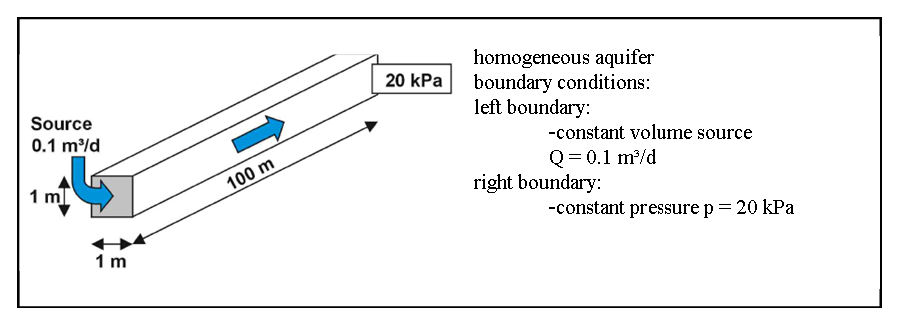
\includegraphics[width=1.0\textwidth]{H_GW/figures/fig21.eps}
\caption{Calculation area: homogeneous aquifer (Ma{\ss}mann, 2004)}
\label{fig21}
\end{figure}

\textsl{Assumptions}

\begin{tabbing}
\=xxxxxxxxxxxxx  \=xxxxxxxxxxxxxxxxxxxxxxx \kill
\> Aquifer: \> homogeneous, saturated, stationary flow
\end{tabbing}

\subsubsection*{Model set-up of the 1~D numerical model}

For the 1-dimensional calculation the calculation area is simplified as a line of a length of 100~m. The calculation model includes 100 elements and 101 nodes. As boundary condition the source volume of the fluid phase of 0.1~m$^3$/d is given at the left border of the calculation area and the constant pressure of 20~kPa at the right boundary. The used parameters of the soil are listed in table \ref{tab21}.
\begin{table}[htbp]
\centering
\begin{tabular}{|c|l|l|}
\hline
parameter & value & unit \\
\hline
porosity $\Phi$  & 0.2 &  --  \\			
\hline
permeability $\kappa$ & 1.0$\cdot 10^{-12}$ & m$^2$ \\
\hline
\end{tabular}
\caption{Used parameters}
\label{tab21}
\end{table}

\subsubsection*{Evaluation method}

The constant flow rate $v_f$ is calculated by using equation \ref{eq23}. In order to calculate the pressure at the left border of the calculation model, Darcy's Law is applied in the following way. The second relation (eq. \ref{eq24}) shows that the pressure gradient is linear.
\begin{equation}
i\,=\,\frac{Q}{k_f\cdot A}\,=\,
\frac{Q}{K\cdot\frac{\displaystyle{\rho\cdot g}}{\displaystyle{\eta}}\cdot A}\,=\,
\frac{1.157\cdot 10^{-6}\,\frac{\displaystyle{\mathrm{m}^3}}{\displaystyle{\mathrm{s}}}}
{9.81\cdot 10^{-6}\,\frac{\displaystyle{\mathrm{m}}}{\displaystyle{\mathrm{s}}}\cdot 1\,\mathrm{m}^2}
\quad\mathrm{and}\quad
p_{\mathrm{left}}\,=\,p_{\mathrm{right}}\,+\,\rho\cdot g\cdot i\cdot l
\label{eq24}
\end{equation}

\begin{figure}[htbp]
\centering
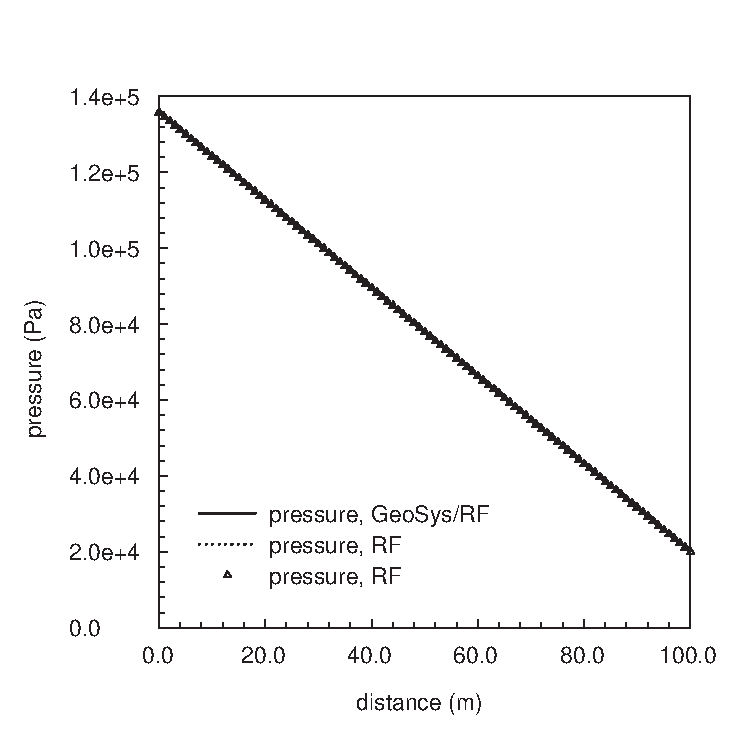
\includegraphics[width=0.5\textwidth]{H_GW/figures/fig22.eps}
\caption{Pressure distribution over the distance of 100~m}
\label{fig22}
\end{figure}

\subsubsection*{Results}

In figure \ref{fig22} you can find the pressure distribution over the whole length of the 1~D model that was calculated by GeoSys/RockFlow. In addition, the analytically calculated pressure distribution is depicted in this figure. These pressure values match the numerical results well.

\begin{tabular}{|l|l|l|}
\hline
Benchmark & Problem type	& Path in benchmark deposit \\
\hline	
h\_sat\_flow\_1d	& H	& benchmarks $\backslash$H$\backslash$sat\_1D \\
\hline	
\end{tabular}
